\documentclass[journal]{vgtc}                % final (journal style)

\ifpdf%                                % if we use pdflatex
  \pdfoutput=1\relax                   % create PDFs from pdfLaTeX
  \pdfcompresslevel=9                  % PDF Compression
  \pdfoptionpdfminorversion=7          % create PDF 1.7
  \ExecuteOptions{pdftex}
  \usepackage{graphicx}                % allow us to embed graphics files
  \DeclareGraphicsExtensions{.pdf,.png,.jpg,.jpeg} % for pdflatex we expect .pdf, .png, or .jpg files
\else%                                 % else we use pure latex
  \ExecuteOptions{dvips}
  \usepackage{graphicx}                % allow us to embed graphics files
  \DeclareGraphicsExtensions{.eps}     % for pure latex we expect eps files
\fi%

%% it is recomended to use ``\autoref{sec:bla}'' instead of ``Fig.~\ref{sec:bla}''
\graphicspath{{figures/}{pictures/}{images/}{./}} % where to search for the images

\usepackage{microtype}                 % use micro-typography (slightly more compact, better to read)
\PassOptionsToPackage{warn}{textcomp}  % to address font issues with \textrightarrow
\usepackage{textcomp}                  % use better special symbols
\usepackage{mathptmx}                  % use matching math font
\usepackage{times}                     % we use Times as the main font
\renewcommand*\ttdefault{txtt}         % a nicer typewriter font
\usepackage{cite}                      % needed to automatically sort the references
\usepackage{tabu}                      % only used for the table example
\usepackage{booktabs}                  % only used for the table example

\usepackage[dvipsnames]{xcolor}
\usepackage{enumitem}

\onlineid{0}

\vgtccategory{Research}

\vgtcpapertype{system}

%% Paper title.
\title{DSOC: Decision Support for Organizational Change}

\author{Rob Barwell and Eric Spero}
\authorfooter{
%% insert punctuation at end of each item
\item
 Rob Barwell and Eric Spero are with Carleton University. E-mail: rob.barwell/eric.spero@carleton.ca.
}

%other entries to be set up for journal
\shortauthortitle{Biv \MakeLowercase{\textit{et al.}}: Global Illumination for Fun and Profit}
%\shortauthortitle{Firstauthor \MakeLowercase{\textit{et al.}}: Paper Title}

\abstract{
DSOC is a novel way to visualize the complex problem of organizational change by allowing the user to quickly see where gaps exist in an organization, understand the gaps that exist, and help the user determine how they might fill the gaps.  This is supported by using email within an organization to model the flow from one employee to another.  This representation provides the most current and concrete representation of the organization and allows the user to make better decisions when faced with organizational change.
} 
\keywords{Organizational change, decision-making, information visualization}

%% ACM Computing Classification System (CCS). 
%% See <http://www.acm.org/class/1998/> for details.
%% The ``\CCScat'' command takes four arguments.

\CCScatlist{ % not used in journal version
 \CCScat{K.6.1}{Management of Computing and Information Systems}%
{Project and People Management}{Life Cycle};
 \CCScat{K.7.m}{The Computing Profession}{Miscellaneous}{Ethics}
}

%% Uncomment below to disable the manuscript note
\renewcommand{\manuscriptnotetxt}{}

\teaser{
  \centering
  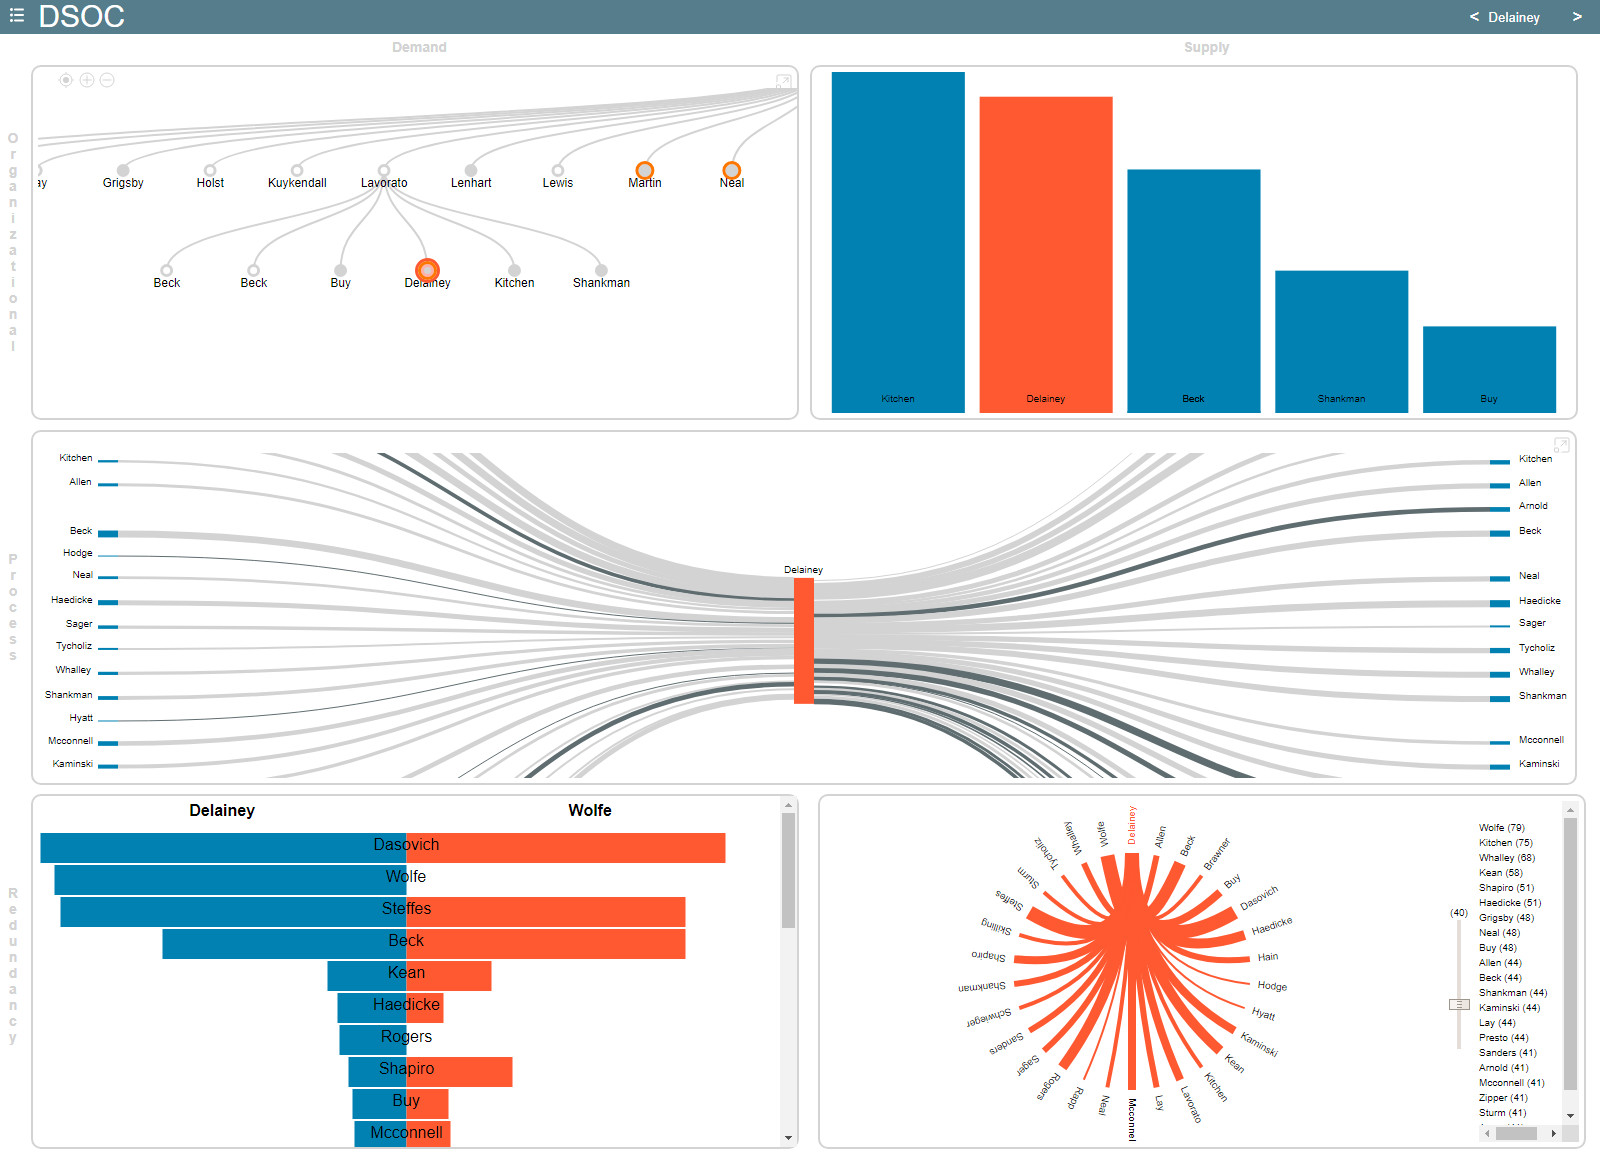
\includegraphics[width=\linewidth]{pictures/version3.jpg}
  \caption{Version 3 of DSOC. Columns: Demand (left) and Supply (right). Rows: Organizational (top), Process (middle) and Redundancy (bottom).}
	\label{fig:version3}
}

%% Copyright space is enabled by default as required by guidelines.
%% It is disabled by the 'review' option or via the following command:
%\nocopyrightspace

\vgtcinsertpkg

%% Start document!

\begin{document}

\firstsection{Introduction}

\maketitle


The rise of the \lq gig economy\rq{}~\cite{de2015rise,friedman2014workers} has forced society through a massive transition in the past two decades with people transitioning between jobs with greater frequency.  Historically, a person would obtain a job from high school or university and stay with a specific company until they retire.  This resulted in organizations that had minimal change, which could be easily managed. Modern organizations are forced to adapt with the shift to the gig economy and other non-traditional employment models.  

An organization is a social network~\cite{scott1988social} of individuals engaged in complex \emph{interlocking contingencies}~\cite{glenn2006complexity}: individuals in an organization are tightly interconnected, where the behaviour of one both depends on, and has subsequent consequences for the behaviour of others~\cite{glenn2006complexity}. This feature of organizations means that the results of changes to its social structure---say, by adding or removing an individual---can be difficult to understand. Change is disruptive, and care must be taken to minimize any negative side-effects. The challenge of minimizing organizational disruption as a result of personnel change depends critically on understanding the effects of that change. In the gig economy, this challenge, and the need for tools that support it, is even greater.

Providing support to organizational change is a complicated problem which has many facets.  The first part of the problem is developing an organizational model that is current and makes sense to the user.  Traditional organizational charts are quickly out dated and do not capture the true nature of the employees contribution to the organization.  This paper will explore a new way to model organizational structure using the flow of emails through an organization along with visualizations to represent this flow and highlight gaps.

During the course of development, as a result of our conversations with others and our own observations, we noticed that the problem of organizational change boils down to a problem of \emph{demand and supply}. When an individual leaves or is removed from an organization, this creates a need (i.e. a gap, a \emph{demand}) which must be addressed by the manager. To do so, the manager will have to inspect their internal pool of resources (i.e. their \emph{supply}) and assign new duties/responsibilities to one or more people.

An individual's function within an organization can be viewed using different lenses. For example, employees can be viewed in terms of their position in the hierarchical structure of the organization, the processes they participate in, and their process- and organizational-agnostic social ties. When dealing with an organizational change issue, the manager should be considering each of these views (and perhaps others not mentioned) on both sides of the demand and supply issue mentioned above.

We present DSOC (Decision Support for Organizational Change), a visual analytics dashboard to help managers respond to organizational change in a way that minimizes disruption to the organization. A screenshot of our functional prototype is shown in Figure~\ref{fig:version3}. When using DSOC, managers are shown a number of visualizations that each help managers grapple with a part of the complex demand and supply problem. Visualizations are organized into two columns: demand and supply, and as many rows corresponding to the views of an employee that a manager is interested in. We implement demand and supply visualizations for three views: \emph{organizational}, \emph{process}, and \emph{redundancy}, which correspond to the three example views mentioned in the example above. 

The structure of the paper is as follows. We cover relevant concepts and related work in Section~\ref{sec:litreview}. In Section~\ref{sec:design} we describe the design of DSOC with an emphasis on how this design evolved over time. We also include background information on our development approach, the domain problem and solution, and our data model. In Section \ref{sec:implementation} we describe how we implemented our design, and challenges we faced along the way. In Section~\ref{sec:evaldiscuss} we describe the use case we presented to users, and provide a walk through of how a manager might use DSOC to help address the issue of an employee leaving an organization in a real-life setting. In Section~\ref{sec:future} we mention a few possible avenues for extending and enhancing DSOC in future work. Finally, we present concluding remarks in Section~\ref{sec:conclusions}.

\section{Literature Review}
\label{sec:litreview}

\subsection{Information Visualization and Cognition}

We aim to address this problem through \emph{information visualization}. Visualizations support thought by reducing the gap between the data, and the users' \emph{mental model} of the data~\cite{yi2007toward}. A mental model is an internal representation of how something in the world works~\cite{staggersmodel,norman2014some}. Wherever there is distance between the presentation of the data and our understanding of the data, mental work must be done so that understanding is possible. This type of mental work does not bring us closer to solving domain goals, but rather is a sort of unfortunate precursor for the really important work, and therefore should be avoided wherever possible~\cite{paas2003cognitive}. Fortunately, the physical environment can be used to store information, which allows us to \lq off-load\rq{} mental work onto the environment~\cite{wilson2002six}. Visualizations are essentially one way of effectively leveraging this property of the environment to aid thought.

\subsection{Related work}

In our review of the literature we found two past projects that tried to address the same high-level problem, organizational complexity, by developing software tools that provided visual representations of the organizations. These two tools differ from DSOC in key ways. Most importantly, neither were designed to help managers fill gaps that were created as a result of an employee's departure from the organization. 

\subsubsection{EnCompass: Organizational Process Visualization}

Mann~\cite{mann1999organizational} recognizes that the day-to-day operations in an organization can have little to do with its organizational reporting structure. He developed a tool called \emph{EnCompass} to help understand the relationships between individuals and the business activities they partake in. Two visualizations of the organization are provided: an ``organizational view'' and an ``issue view''. The ``organizational view'' is a 3D representation of an organization's reporting structure. The ``issue view'' is a 3D tree of all employees involved in a given process. The level the employee is placed at is determined by their important to the process, as determined by a questionnaire completed by employees. For each view, networks of process-specific employee interactions can be superimposed on the trees.

EnCompass and DSOC both address the same high-level problem: the day-to-day operations of an organization are difficult to understand, and often unknown. We both try to address the first of these problems with information visualization. We differ in terms of how we address the second issue: EnCompass gathers detailed process-specific data from questionnaires issued to employees, whereas DSOC uses a simple value model of SMTP headers.

The specific lower-level problem the two tools target, however, are rather different. EnCompass is meant to help align an organization's reporting structure with its business processes (i.e. ``day-to-day operations''), whereas DSOC is meant to help managers fill gaps left by an employee's departure from an organization. Providing visualizations that specialize in showing supply and demand information respectively give DSOC an advantage in this task, and there is no equivalent functionality in EnCompass.

\subsubsection{Perspective Oriented Business Process Visualization}

Perspective oriented business process visualization (POBPV) is a ``flexible and extensible meta model'' providing multiple perspectives on a business process model to help users better understand complex business processes. This tool provides visualizations for five perspectives of a business model: functional, data, operational, organizational, and control flow/behavioural. 

POBPV and DSOC both apprecite the complexity of organizations, and try to make them more understandable by leveraging the power of information visualization. Both tools provide multiple perspectives on the problems they are designed to address using a set of visualizations each applied to a different perspective.

However, the two tools are targeted at quite different problems. The focus in POBPV is on understanding business processes, not employees. It is difficult to imagine a manager using this tool to address organizational change, as employees are only directly represented in one of the five views (organizational). POBPV also uses much simpler visualizations: simple hierarchies, flow charts, and UML diagrams, perhaps because rich and interactive visualizations were more difficult to implement when the tool was designed. 

\subsection{Enron Corpus}

As a result of the infamous investigation into the Enron corporate scandal, the Federal Energy Regulatory Commission subpoenaed Enron's email records. Later, these records were made available to the public, and since have become one of the most valuable datasets for research~\cite{networkanalysis2015hardin}. 

The use of the Enron corpus in research is ``prolific and wide-ranging''~\cite{networkanalysis2015hardin}. For example, it has been used by social network analysts to: detect social hierarchies~\cite{rowe2007automated}, to study how patterns of communication shifted between normal operations and the crisis stage~\cite{diesner2005communication,diesner2005exploration},  to find out the topics of emails and the social roles of the communicators~\cite{mccallum2007topic}, and to find patterns between word use and role within the organization~\cite{keila2005structure}. A team of researchers at Berkeley created a suite of visualizations to help reveal insight into the social networks at Enron~\cite{heer2005exploring}. 

We were not able to find prior attempts to use the Enron database as part of a visualization tool to help managers make decisions. 

\section{Design}
\label{sec:design}

Our design is built on top of two key ideas:

\begin{enumerate}
\item The problem of dealing with an individual leaving an organization is in essence a problem of \emph{supply} and \emph{demand}. 
\item An individual's role in an organization is \emph{multifaceted}: it is different depending on the \emph{view} one takes.
\end{enumerate}

When an individual leaves an organization, a gap has been left (or a demand has been created), which needs to be filled. The manager responsible for addressing this issue will first need to take note of what and where the gaps are. Then, they will look at the remaining members of their organization to find ways of filling those gaps.

The problem is that there are a number of different kinds of gaps, pertaining to each of the facets, or views, of the individual's role. These views are often not reflected in the person's job description, and they might be unknown, or difficult to find out. The supply and demand problem spreads over all of these views. This problem is duplicated when looking through one's supply for replacements, as their roles are equally difficult to know.

Our interface is meant to visualize the \emph{demand} created by an individual's departure from an organization for each facet of their role. Alongside the visualizations of the demand created, we want to explore the space of potential replacements, visualizing their roles as well.

In the remainder of this section, we discuss the various elements of our design in more depth, tracing its evolutionary history through several versions, and providing rationale for our design decisions.

\subsection{Background}


\subsubsection{Methodology}
\label{sec:methodology}

The development of our visualization started with defining a methodology to help guide the design process.  We reviewed a number of papers in the area of evaluation of information visualization.  We found this area of research to be less concrete then other topics we had studied before.  The Challenge of Information Visualization Evaluation~\cite{challengeofinfoviseval} paper we reviewed helped us to clarify our evaluation criteria and approach by validating our desire to present our design and findings to various user groups throughout the design process.  The Empirical Studies in Information Visualization: Seven Scenarios paper~\cite{lam2012empirical} paper inspired us to take an iterative approach, similar to agile software development.  The approach presented in the paper was Pre-design, design, prototype, deployment, and re-design.  This approach would also line up with using different user groups through the process.

Our design was informed by consultation with three user groups. Those groups are:

\begin{enumerate}[label=(\Alph*)]
\item  \textbf{Government Department}. Members of a large department at the Government of Canada who address organizational change issues in their work.
\item \textbf{Academia}. Students and a professor at Carleton University.
\item \textbf{Private Company}. Users at a private multi-national company who discovered our research during the design process.
\end{enumerate}

We made the real-world viability of our design a top priority. As such, we felt it was important to show our design to people from a number of different backgrounds to help ensure that our design was comprehensible to a wide variety of potential users, and that our visualizations effectively communicated the underlying data and helped support the task at hand. Our initial design underwent two major revisions in response to feedback received from members of these groups. 

After implementing Version 1 (V1) of our prototype we presented it to Group A. Group A provided the key insight that the problem we were addressing was a problem of demand and supply across multiple views. The design concept behind V2 (a major redesign) came directly from our interactions with Group A. V2 was then shown to Group B, who pointed out a number of issues with specific visualizations.  This group provided creative ways of helping support the needs identified by Group A. V3 was then shown to all groups, where no major issues with our implementation were identified.  {color{gren} V3 allowed the discussion to evolve past the visualization into how it would help each group take the problem of organizational change.}

\subsubsection{Problem Space}
\label{sec:problem}
After implementing our original design and going through several subsequent iterations, the way in which we framed the core problem we were trying to address also changed. We loosely followed Pirolli and Card's sensemaking loop~\cite{pirolli2005sensemaking}: we started with a question, eventually leading to a hypothesis, and then through a validation process, leading us back to a new formulation of the question.  

The problem as we originally conceived it was simply how to help managers fill empty positions in the gig economy era, which has high employee turnover. Managers rely on organizational models like organizational charts to help with this task, which are representations of the structure and function of an organization. Organizational charts are not ideal tools for this task as they are quickly out of date in the gig economy, and they provide a limited view of a person's role in an organization. We set out to offer a new solution leveraging the power of graphical user interfaces and information visualization. 

As we developed our design, we found it useful to break our original definition of the problem into sub-problems. Each sub-problem imposed their own demands on the interface, which were lost in the original definition. We eventually recast the original problem into three research questions: 

\begin{enumerate}
\item “How do we support decision makers to minimize negative side-effects from organizational change?”
\item “How do we value a person in the organization?”
\item “How do we provide options to users to address vacancies within an organization?”
\end{enumerate}

From the point of view of the manager, these questions take the following form: 

\begin{description}


  	\item [``Where is the gap?''] Gaps left when an employee leaves are not restricted to the employees organizational group, but could effect other groups as well.  Job descriptions are typically a poor reflection of an employees job as they are only updated when an employee leaves.  This means Eric in our example needs to look at the organizational side of the problem and the process side of the problem.
	\item [``How big is the gap?''] When gaps are found the manager needs to know are they small such as a person just needs to sign an approval form, or are they big such as the person who is responsible for producing a yearly financial report.

	\item [``What can I do about the gap?''] This problem is the most complex as it require the manager to evaluate first if they are filling the gap and then what resources do they have available to them to fill the gap.
\end{description}

\subsubsection{Option Space}
Using a refined problem description we started to focus on how we would address these statements.  Using the work done by Ware on Visual Thinking Algorithms~\cite[Chapter 11]{ware2012information} we decided to enumerate the steps a user would do manually to solve the problem statements and determine where visualization could help offload cognitive processes.

During our walk through of V1 with Group A, we presented V1 of the interface and asked users to imagine using the software to solve the original problem. Group A immediately sub-divided the problem into the three sub-problems mentioned in Section \ref{sec:problem}, and explored it from different perspectives or views. Group A expressed that it would be helpful if the interface could model all of the different views. The different views are summarized below:

\begin{description}
\item [Organizational] This places an employee in the traditional hierarchical organizational structure.  Commonly this is represented by a tree where the employee is a node and an edge is the link between nodes.
\item [Process] This places an employee as part of a process where they receive information, process information, and output information to the next stage of the process.  Users typically used flow charts and other process diagrams to represent this view.
\item [Redundancy] During the walk through we noticed it was most common to address the vacancy by re-distributing the workload within the group, however the users occasionally tried to find people that did similar tasks as replacement.
\end{description}
\begin{figure}
  \centering
  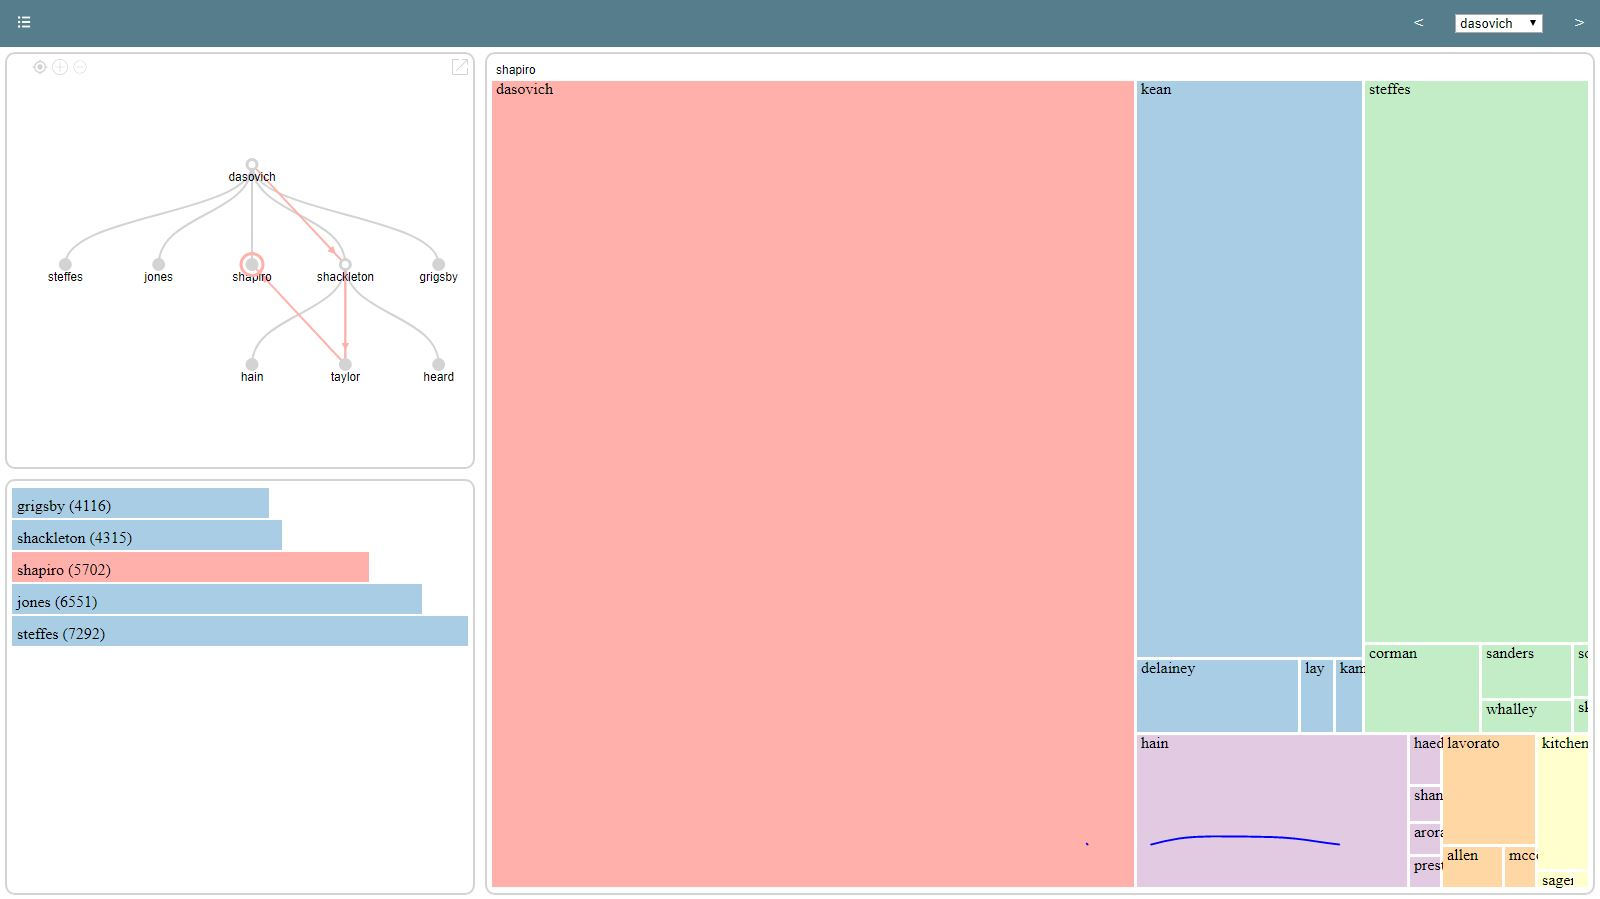
\includegraphics[width=\columnwidth]{pictures/version1.JPG}
  \caption{Version 1. }
  \label{fig:version1}
\end{figure}
      

\subsubsection{Data}
During the exploration of the problem space we needed to identify what data we were going to present to the user with the visualization.  Building upon an idea from our colleague on information flow within an organization, we decided to use emails.  The majority of communication within a modern organization is through email or instant messaging.  We thought that analyzing email data would allow us to build an accurate and up to date model of how information flows through an organization.  

Using emails as the basis of our data model was well-received by Group A because it addressed some shortcomings with the traditional organizational chart model, which is typically out of date and does not capture all of the contributions an employee makes to an organization.

The data model requires enrichment through the addition of value models.  One value model would be required to help the manager find out ``How big is the gap?'' and another value model would be required to help the manager find out ``What can I do about the gap?''.  We use rudimentary value models as the primary focus of this paper is the problem of how to visualize the data, and not the data itself.

\begin{description}
\item [Gap Size] By modeling each employee as a node, the emails between nodes would represent an edge with a weight of 1.
\item [Gap Options] One option to address the gap could be redistributing the work to a \lq similar\rq{} employee. The value model we used to compare the similarity of two employees is \lq overlap\rq{} in terms (a) number of emails sent, and (b) who the emails are sent to.
\end{description}

\begin{figure}
	\centering
	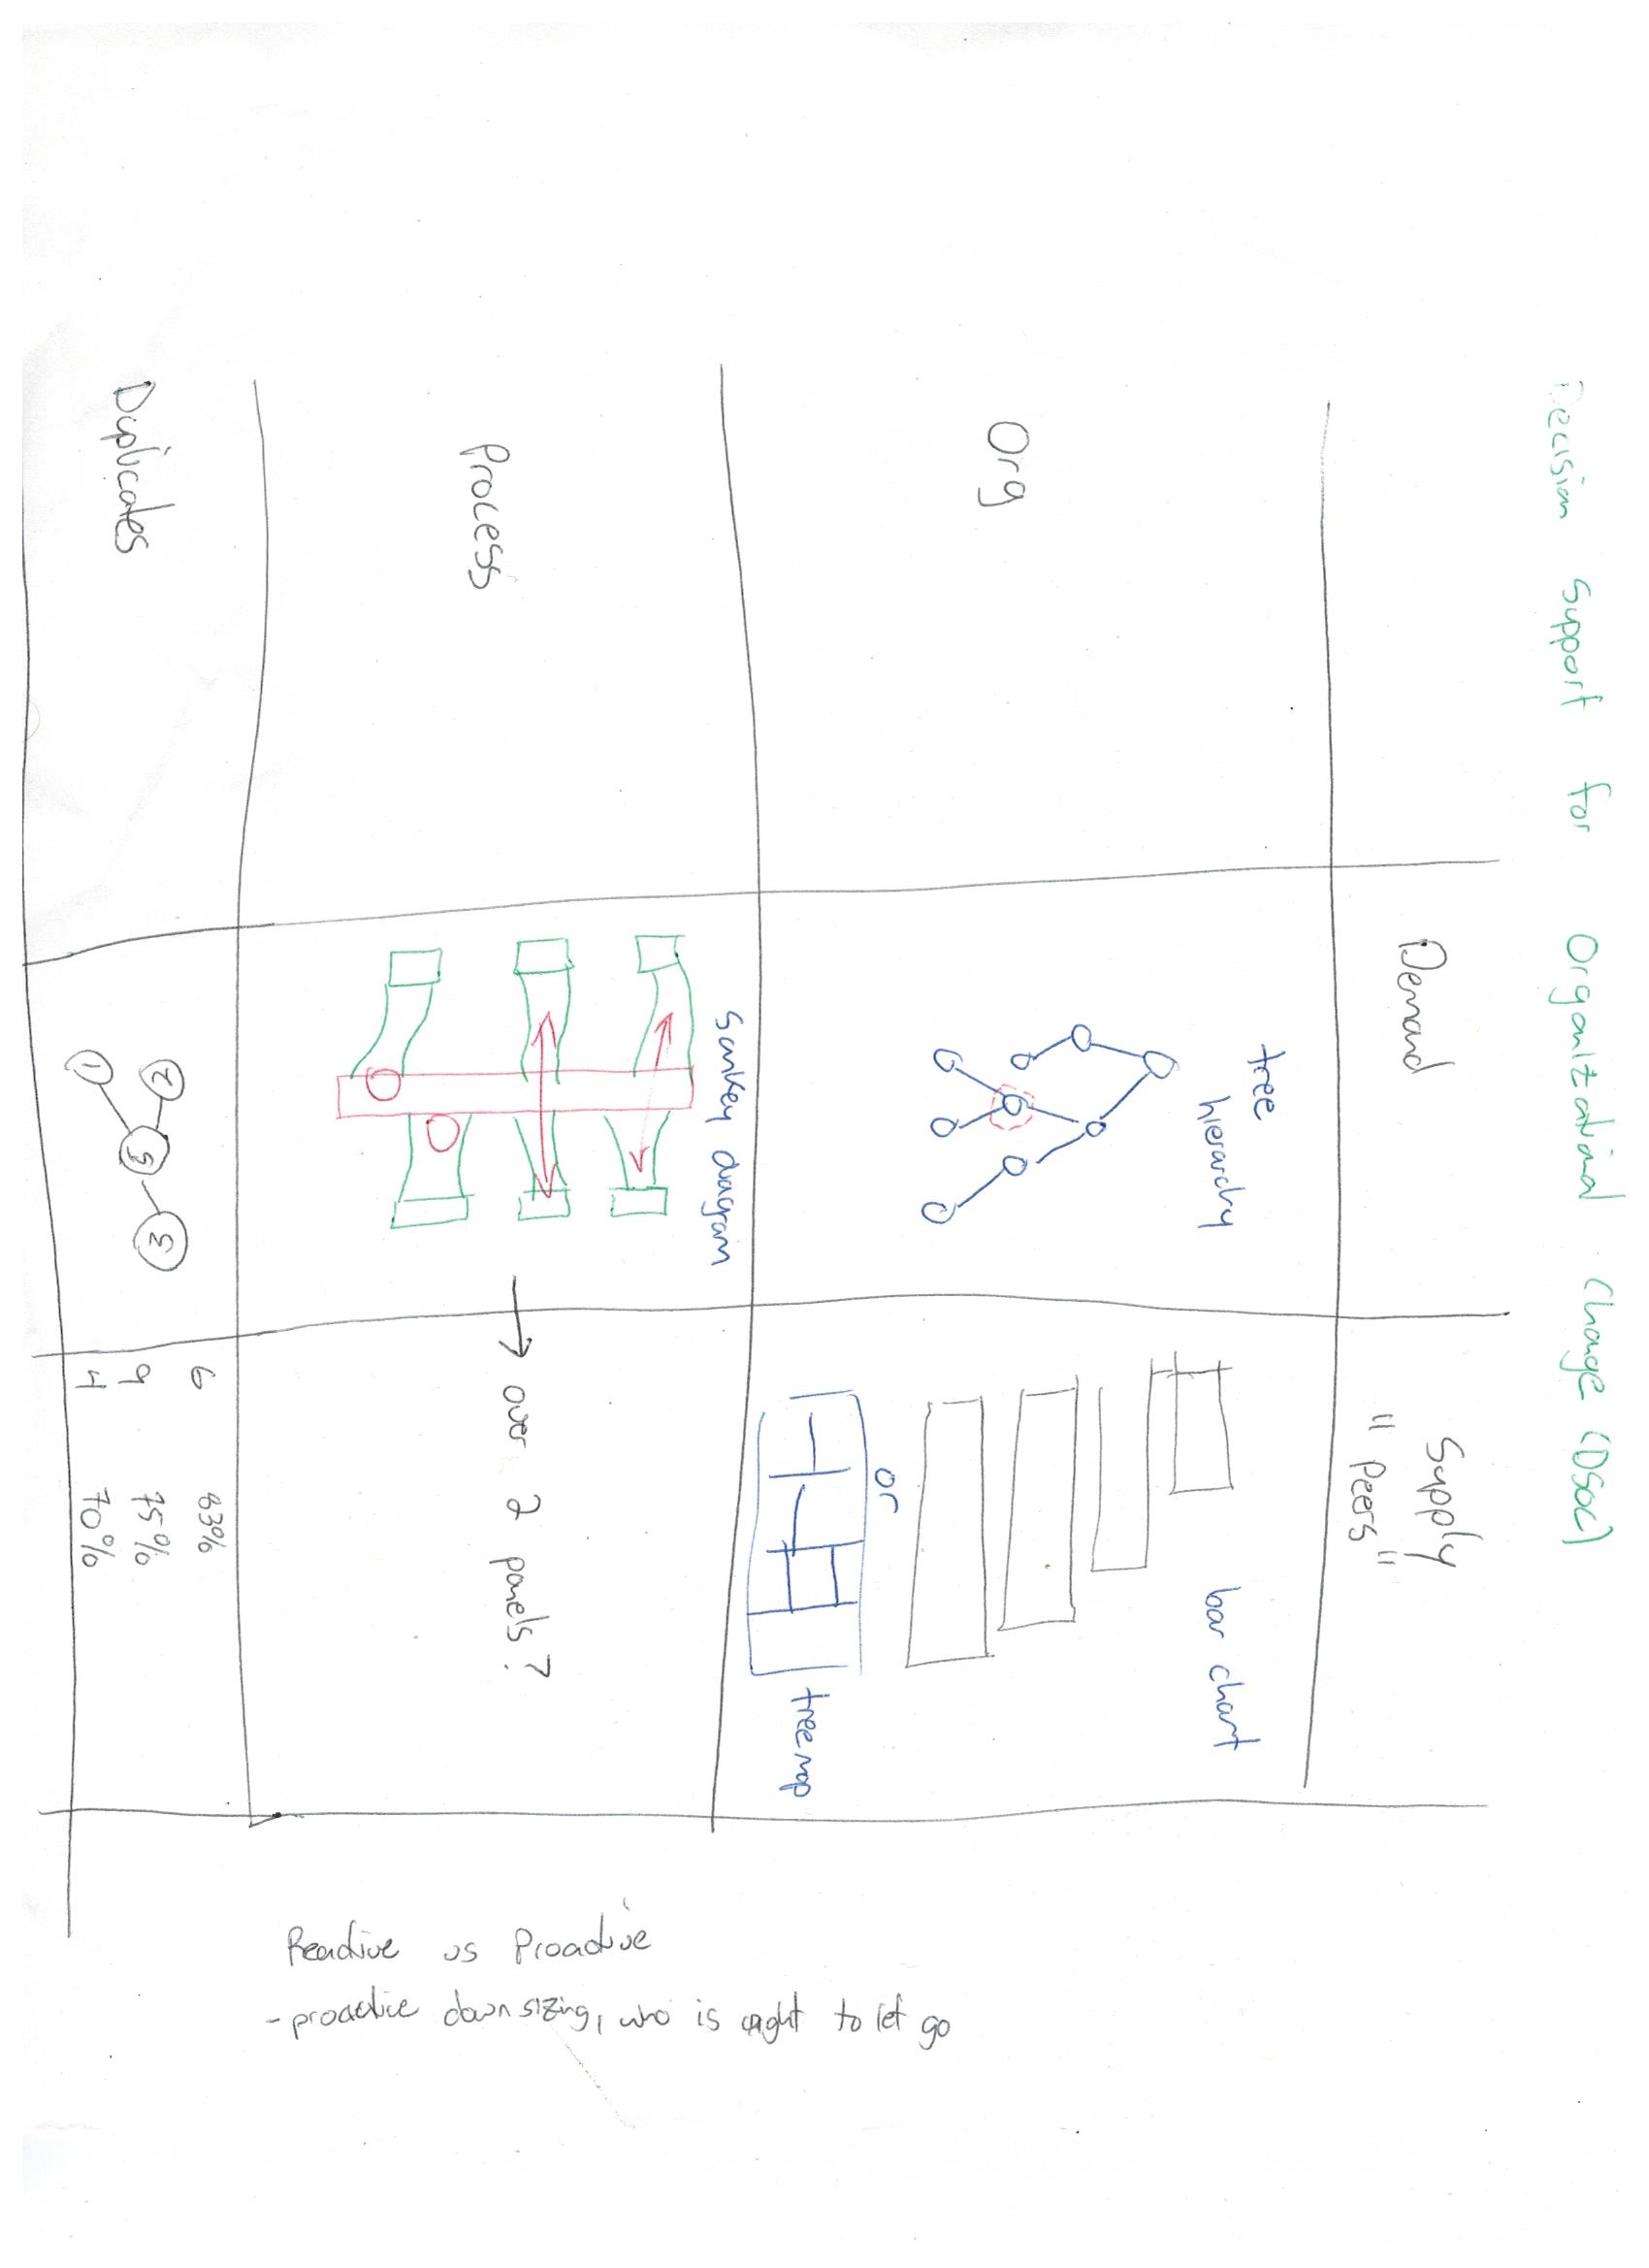
\includegraphics[width=\columnwidth]{pictures/Sketch.jpg}
	\caption{UI design sketch drawn after initial meeting with Group 1. Shows the grid pattern and several of the visualizations used in the final version.}
	\label{fig:sketch}
\end{figure}

\subsection{Major Versions}

The incremental refinements to our design in response to feedback obtained from the users in the groups mentioned in Section \ref{sec:methodology}. Our design went through three major versions:

\begin{enumerate}
	\item [\textbf{V1}] Figure \ref{fig:version1}. Initial attempt at solving the problem. 
	\item [\textbf{V2}] Figure \ref{fig:version2}. Overhauled layout, and introduced \emph{demand-supply $\times$ views} grid layout. Added the process and redundancy views.
	\item [\textbf{V3}] Figure \ref{fig:version3}. Refined the process and redundancy views to better align with the users' mental model and how they interact with the visualization.
\end{enumerate}

Our greatest challenge was creating a functional and comprehensible layout that also conveyed the complex intricacies of organizational change.

\subsection{Layout}
Here we discuss the structure of our layout and how it is navigated. 
\subsubsection{Structure}
The original design, shown in Figure \ref{fig:version1}, had  viewing panes to try and convey the organizational perspective of information flow and the process perspective.  It attempted to do this using the standard organizational tree for organizational structure and a tree map to show the volume of communication between a selected individual and their communication links.

This view presented many challenges for users as they found it difficult to understand what the visualization was trying to communicate. There seemed to be a severe incompatibility between this design and Group A's mental model of the problem of organizational change. For Group A, the problem at hand boiled down to a problem of \emph{supply} and \emph{demand} (these were the words they used most frequently during this conversation), yet these concepts were not straightforwardly represented in our design. This observation called for a major redesign of the structure, where starting in V2 (Figure \ref{fig:version2}) we would build the notion of supply and demand into our structure. The first stage in this redesign is captured in the sketch in Figure \ref{fig:sketch}.

The new design featured a grid layout of 2 columns $\times $ $N$ rows. Visualizations that focus on the \emph{demand} aspect of the problem are placed in the left column, and visualizations focusing on the \emph{supply} aspect are placed in the right column. By visualizing both the supply and demand aspects of the problem next to each other, managers can simultaneously see the gaps left by an individual's absence, and also ways to fill those gaps.

Visualizations for the different views of the problem space were each placed inside their own row. We say there are $N$ rows because there is no theoretical upper limit to the number of views that a manager may want to examine. The views that a manager may want to examine can vary based on the demands of the specific situation they are in. We provide three example views, but more can be created and added to the dashboard as needed.

We found that visualizing each view of the problem space separately had a similarly positive effect as visualizing supply and demand. 

\begin{figure}
	\centering
	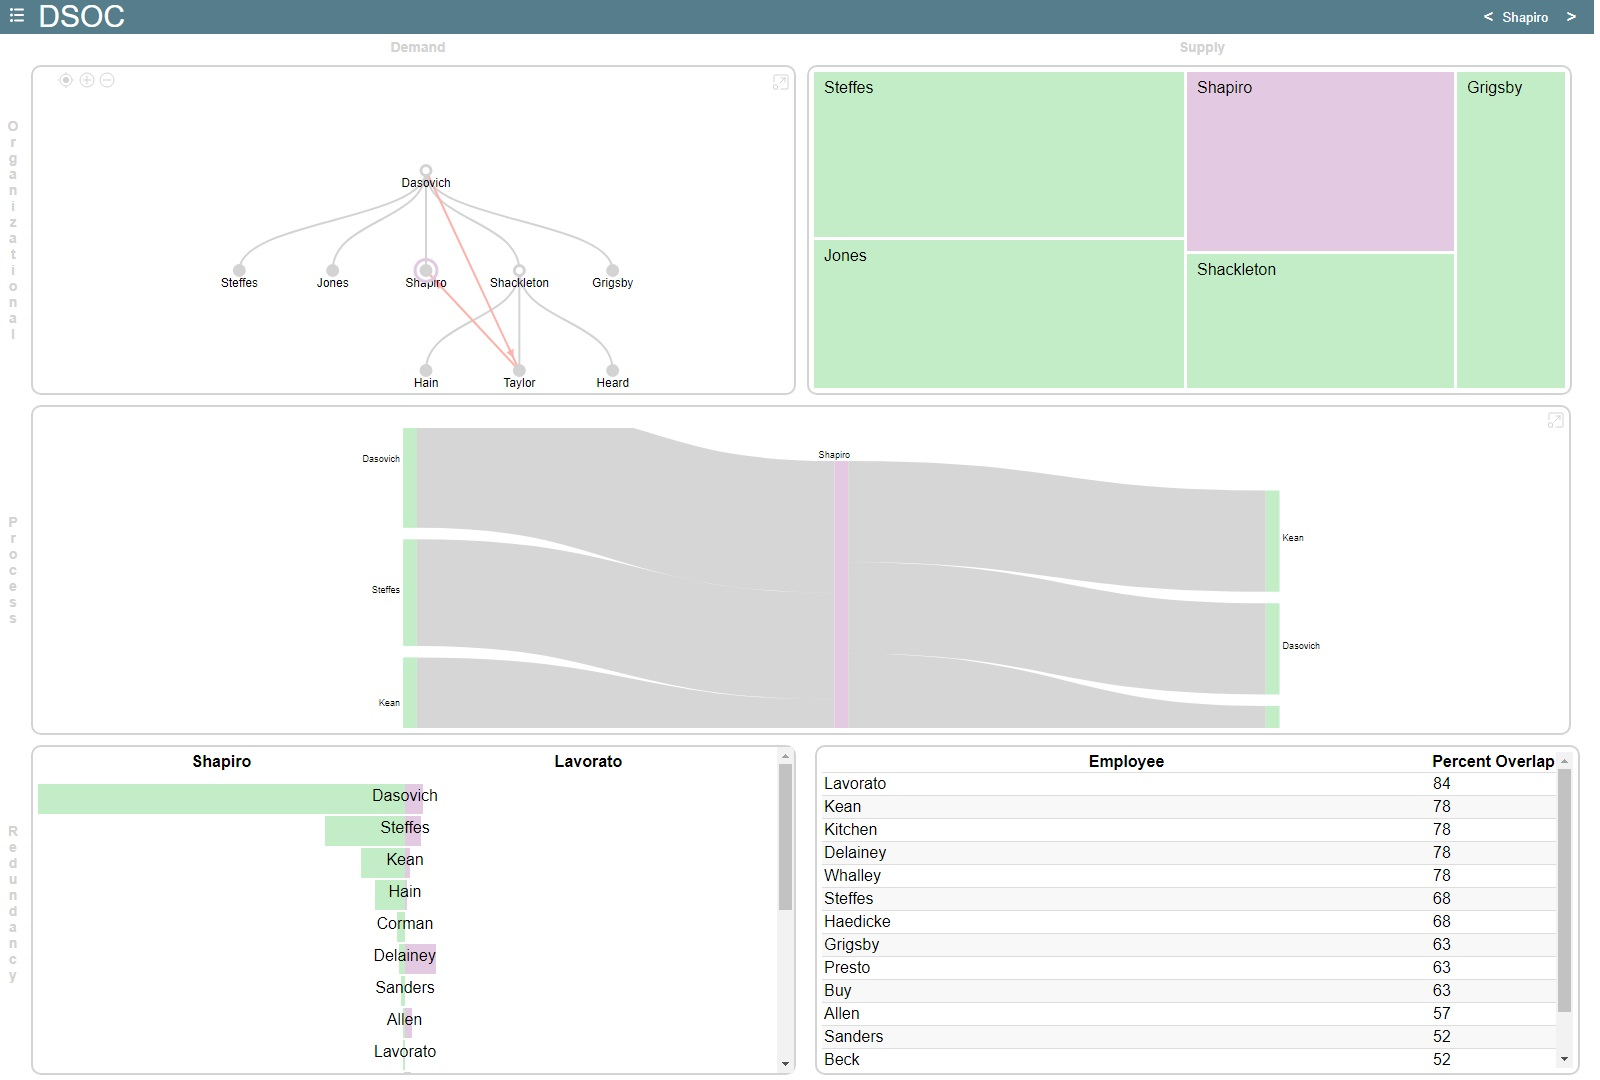
\includegraphics[width=\columnwidth]{pictures/version2.jpg}
	\caption{Version 2}
	\label{fig:version2}
\end{figure}

\subsubsection{Navigation}

Our goal was to provide the user with the freedom to explore the problem space however they choose.  This required the support of a brushing scatter plot concept where the interactions within an individual sub-view are reflected in the other sub-views. The visualizations are all driven by the \emph{selected} node: users view a single data point through a number of lenses. Users can select a node by clicking on nodes in either of the ``Organizational'' views. 

As the user explored the problem it was also important to have a way for them to keep track of the problem space they have already explored.  This was a salient point that we found during the literature review with the quote ``Information exploration is inherently a process with many steps, so keeping the history of actions and allowing users to retrace their steps is important''\cite{anafigueiras}.  This was included by providing the user the option to display history as direction arrows or simply colouring the nodes in the organizational chart.  The user can then navigate the history using the navigation bar at the top of the screen.

\subsection{Views}
We provide three views of an employee's role in an organization: \emph{organizational}, \emph{process}, and \emph{redundancy}. The \emph{organizational} view is the employee's position in the organization's reporting structure; the \emph{process} view suggests the processes they participate in, with an emphasis on whether they are at the start, end, or middle of a process; and the \emph{redundancy} view considers their pattern of communication with other individuals in the organization.

In this section we describe how we represent these views in DSOC, and how this changed through the major versions.

\subsubsection{Organizational}
The organizational demand and supply view changed relatively little between V1 and V3 compared to the other visualizations.  The org-demand view was modeled after a classical organizational tree structure, as this paradigm was most aligned with the users current mental model of the problem.  During the design phase we uncovered a number of issues that we needed to address, which we discuss next.

\paragraph{Actions}
Organizational trees can be quite large, so we need to provide the user with the ability to zoom in and out of the tree, expand and collapse a node's children, and focus on a specific node.  In V1, a single click both expanded a node's children and selected the node; double-click would zoom in and out of the tree.  Users in Group A complained about this, and wished to expand a node without selecting it and vice versa. These functions were separated more cleanly in V2, where a single click selected a node, the double click would zoom in and out, and a right mouse click would open a node with children.

\paragraph{Highlight}
During the initial design of V1 we needed to come up with a creative solution to visualize the various states a node could have.  This includes: being selected, having children, being visited, and being filtered.  We originally experimented with glyphs and other icons, however the resulting visualization was too busy.  We settled on using concentric circles of different colours to denote various states of a node. The concentric circles can be seen in Figure \ref{fig:node}  A node with children has a filled in circle; nodes the user has visited have a faint orange outline; nodes that are filtered have a darker orange ring around the outline of the main circle; and the selected node has an even larger red ring around the previous ring.  

\paragraph{Navigation}
Navigating large trees can present challenges for users.  One way we help users navigate large trees is with a real-time filter. Users can adjust the filter parameters, and the nodes that meet the filter requirements are highlighted with an orange circle, distinguishing them from non-filtered nodes.  Users can also expand the organization demand panel to fill the whole window so users can see more of the tree at once. Icons at the top of the frame provide navigational short-cuts allowing the user to center on the current selected node, expand all nodes, or collapse all nodes.

\paragraph{Comparison}
When users hover over a node, a blue line is drawn from that node to all the nodes they communicate with. This allowed users to see at a glance everyone a given individual talked to. Originally the strength of the connection between two nodes was not communicated to the user. In later revisions, after discussions with Group B, this feature was changed to communicate the strength of the connection through the thickness of the blue line connecting the two nodes, where a thicker line meant a stronger connection. This feature can be seen in Figure \ref{fig:node}.

\begin{figure}
	\centering
	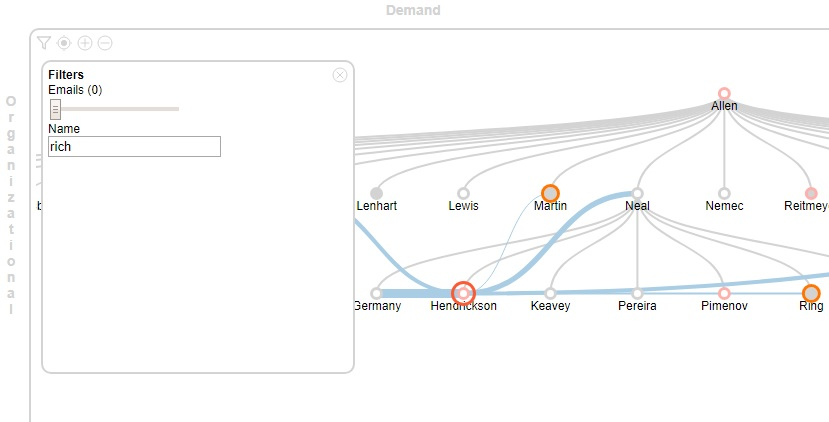
\includegraphics[width=\columnwidth]{pictures/orgdemand.jpg}
	\caption{Node Selection}
	\label{fig:node}
\end{figure}

The organizational supply view was originally a horizontal bar chart, as shown on in the bottom-left pane in Figure \ref{fig:version1}.  In V2 we experimented with changing this to a tree map, as we wanted to show the relative size of each employee in a group compared to the others.  The space filling method~\cite{shneiderman1992tree} as discussed in Ben Shneiderman original treemap paper was appealing as we did not know how large a group might be.  After discussion with Group B we decided treemaps were not appropriate as there were no levels to drill down to or group by.  It was also noted by Group A that a bar chart might be better for a comparison view point.  When the user clicks on any of the bars it will re-orient all views to select the employee.  The final vertical bar chart is shown in Figure \ref{fig:version3}.

\subsubsection{Process}

The process demand and supply visualizations underwent major changes between versions.  In V1 a treemap was used to model the communication flow between the selected employee and those they communicate with.  This approach provided an overview of who the employee talked to and how much. However, Group A noted that this approach failed to give an impression of how information flowed through an individual, nor what processes started or ended with an individual---two things a manager must consider when looking for gaps and ways of filling gaps.  Group A's suggestion was to investigate using a Sankey diagram, which we added in V2.

The Sankey diagram used in V2 and V3 show the selected employee in the center, the employees who send emails to the selected employee on the left, and the employees who the selected employee sends emails to on the right. The relative width of the lines communicates the number of communications sent. Dark lines on the left indicate that the employee talks to the selected employee but not vice versa, and dark lines on the left indicates the reverse. These suggest instances where the selected employee is the start (right) or end (left) of a process. 

The original version of the Sankey diagram in V2, shown in Figure \ref{fig:version2}, was problematic for Group B. The flow lines on the left side of the selected employee (the line in the middle of the diagram) appeared to carry through to the lines on the right, which made it seem as though the information from an employee on the left was transferred directly to an employee on the right by the selected employee. This was an accident of the layout algorithm and not something that we intended to communicate (since we have no knowledge of the content of the emails), and therefore it was misleading.  Additionally, the lines joining employees were typically quite thick which made the visualization hard to read. Also, employees on the left and right were presented in different orders, which made direct input-output comparisons for a given conversational partner difficult. Based on this feedback, we decided to completely redesign this diagram for V3.

For V3, we reduced the appearance of information directly transferring from an individual on the left to an individual to the right through the selected employee by (i) scaling down the width of the links, and (ii) increasing the width of the bar representing the selected individual, helping to convey the impression that the information from the left is not fully continuous with the information on the right.  Scaling down the links also made them easier to differentiate. We added colour to denote links that either started or ended with the selected employee. Finally, we lined up employees that appeared on both the left and right to allow for easier comparison.

The Sankey diagram is unique among the visualizations we use in its ability to communicate both supply and demand simultaneously. This feature will be further discussed in the evaluation and discussion section.

\subsubsection{Redundancy}

The redundancy view was introduced in V2 after our initial discussions with Group A.  They thought it would be a good idea to show similar people within an organization as a potential supply source to fill the identified gap. V2 included a simple implementation of this concept. In the demand pane, a back to back bar chart was used to help the user determine if the supply lined up with the demand. In the supply pane, we provided a table showing the employees who had the most \lq overlap\rq{} with the selected employee, in descending order of percentage of overlap.

Group B expressed dissatisfaction with our decision to show overlap supply with a table. They felt that overlap was an inherently visual concept, and thus demanded a visual representation. This led us to investigate a number of options including hierarchical edge bundling and chord diagrams to try and show the overlap between two selections.  The chord diagram was an unsatisfactory solution as the selected employee filled the entire circle, making it hard to differentiate between the different paths.  The hierarchical edge bundling had the major drawback of not showing the relative size of each connection.  We decided to merge these two concepts together, creating a single visualization: the \lq palm tree\rq{} diagram shown in Figure \ref{fig:palm}.

The palm tree diagram quickly shows how much an employee overlaps with a selected employee in a visual fashion. The diagram shows the selected employee, whose name is written in orange, and all of the employees they communicate with. Their connection is signalled with an orange line, and the width of the line shows the volume of communication between the two parties. A list on the right shows a list of other employees in the organization in descending order of the amount they overlap with the selected employee. A slider to the left of this list allows the user to filter this list by overlap percent. When the user hovers over an employee on this list, their pattern of communication with the employees the selected employee speaks to is drawn with blue lines from the same origin as the selected employee. By rolling the mouse up and down the list, the user can make quick comparisons between employees. We chose the orange and blue colour scheme because we felt it provided the optimal balance between high contrast, allowing the user to easily distinguish between the two lines when performing overlap comparisons, and aesthetics. 

This approach seemed to resonate well with all user groups in V3.  Users appreciated its flexibility in gracefully showing a large number of connections, and its ability to convey overlap information quickly and effectively. 

\begin{figure}
	\centering
	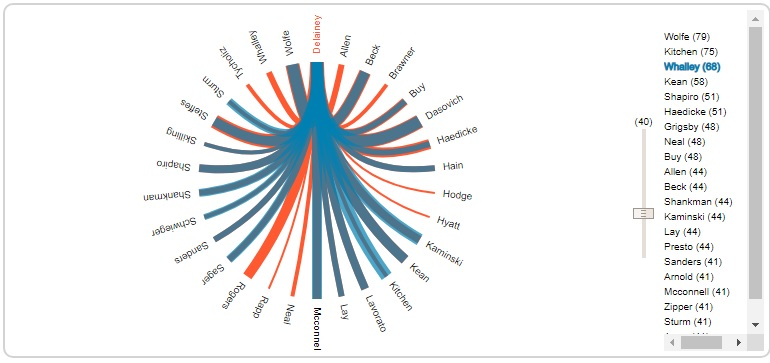
\includegraphics[width=\columnwidth]{pictures/palmtree.jpg}
	\caption{Palm Tree}
	\label{fig:palm}
\end{figure}

\section{Implementation}
\label{sec:implementation}
Each version of the design was implemented using MySQL, PHP, HTML, CSS, and Javascript using the D3 library.  A number of visualization systems were contemplated, however D3 was chosen due to its maturity level and flexibility.

\subsection{Data}
Email (SMTP) header information was used to implement the value model discussed in the previous sections. Extended value models are discussed later in Section \ref{sec:future}.

To demonstrate our value model we chose the Enron email dataset~\cite{cmuenron,klimt2004introducing}. This dataset was originally made public during the Federal Energy Regulatory Commission investigation.  It contains the emails of approximately 150 users in the Enron organization, most of whom are senior managers.  This particular dataset has been frequently used in research, typically with a focus on social networking and natural language processing~(e.g.~\cite{diesner2005exploration}). We use this dataset to illustrate our visualization to support the flow of information through an organization.  

In addition to employee's emails, we also needed an organizational chart, which provides one of the views of an employee's role.  Unfortunately, we were unable to find an official Enron organizational chart, which is a known issue with the dataset.  Since our research is primarily focused on the visualization and not the underlying data, we decided it would be acceptable to use an organizational chart that was reverse-engineered from this dataset by a group from the University of Amsterdam~\cite{rowe2007automated}. Out of a number of different approaches to extracting organizational chart information from the Enron dataset, the approach used by this group seemed to us as the most sophisticated.

\subsubsection{Data Preparation}

The Enron dataset was obtained from Carniege Mellon University~\cite{cmuenron}.  We used a Python script to parse SMTP header information for each email.  We stored this data in a MySQL database, which would be further processed by the application. We chose SMTP information because it contained all the basic information required to construct the nodes and edges within the graph.

\subsection{Organizational}
The organizational view was straightforward to implement. We used the hierarchical tree and bar chart components of D3.  Custom path generation was required to connect nodes upon a mouse hover event, shown in Figure \ref{fig:node}.  This was accomplished by binding the database node id to the D3 object id.  This facilitated the selection of individual nodes in the tree to determine their $x$ and $y$ position to draw a path between.  This process was also used for the history link paths, which can be seen in Figures \ref{fig:version1} and \ref{fig:version2}.

The only design choice that arose during implementation was what to do when two nodes are connected, but one node isn't visible.  In this case we decided to connect the visible node to the closest parent of the hidden node.

\subsection{Process}
The process view was the most complex to implement.  It required a custom written layout generator.  The generator takes a list of all nodes and edges for a current view and then splits the edges into incoming and outgoing.  After iterating through the edges to determine if the incoming or outgoing edge is greater, it conducts a layout which utilizes the full space allocation.  Nodes are also logarithmically scaled to reduce overlap and make the visualization easier to use.

\subsection{Redundancy}
The redundancy view was the most challenging to implement since it had a number of custom visualization components.  A custom bar chart was required to display the back-to-back bars in the redundancy demand view, as D3 only had a standard bar chart.  However, a number of D3 features that create bar charts were utilized to create the back-to-back bar chart.

The most challenging feature to create was the palm tree in the redundancy supply panel.  This required a custom layout that would place the selected employee in a circle with all the people they communicate with.  Then additional layers were placed on top to position the compared employee in place of the selected employee.  This also required a custom data structure to communicate this information from the server to the D3 engine.

\subsection{Other Implementation Choices}

\begin{description}
\item [Colour] A single colour scheme was implemented to ensure consistency across all views.  This provides consistency for the user where all the nodes are the same colour regardless of view, and the selected node is easily identifiable. We chose orange and blue because they are highly contrasting while still looking aesthetically pleasing.
\item[Layout] The layout was implemented using CSS grids that allow for the screen to be divided into frames.  This allowed us to show two full rows no matter the size of the window..
\item[Labels] The new supply and demand layout gave meaning to each row and column. We added labels to explicitly communicate this meaning to the user.  Users found this very helpful to understand the problem space.
\end{description}

\section{Evaluation and Discussion}
\label{sec:evaldiscuss}

Evaluation of the design was done at a number of points during the development. We made many significant changes as a result of feedback from users. In later stages of evaluation, we received direction on future work, and gained some insight into how organizations might use the final product.  During the development we explained our design using a use case to help participants put themselves in the shoes of the intended user, thereby increasing the ecological validity of the results. We describe the use case below. 

\subsection{Use Case Walkthrough}
An employee, Rob, has left a company, and the manager, Eric, has to fill the need this has created. The employee could have left because they switched jobs, they could be on a temporary leave of absence, or they could be seconded to other positions. The manager needs to assess the gap that has been left, and how to fill it. To do this, Eric must seek answers to the three questions we described earlier in Section \ref{sec:problem}:

\begin{enumerate}
\item ``Where is the gap?''
\item ``How big is the gap?''
\item ``What can I do about the gap?''
\end{enumerate}

\subsubsection{Finding the Gap}
Our visualization helps Eric with each of these questions.  First he can identify the gap by using the organizational demand tree shown in Figure \ref{fig:version3}.  By navigating and filtering the tree Eric can start to understand if Rob managed any employees under him. The higher he is on the organizational chart, the more employees in the tree will be without leadership. The tree can also be used to quickly determine which parts of the organization might be effected most, by hovering over Rob and looking where the largest blue lines connect to.

Using the process view, Eric can determine which email connections start or stop with Rob.  This typically denotes starts and ends of processes, which are high-priority gaps to fill.  Additionally, the process diagram can provide Eric an overview of the stronger communication links Rob had, which signal processes Rob was an integral part of.

\subsubsection{Size of the Gap}
During the exploration process in finding the gap, Eric has already started to understand the size of the problem by looking at weight of the lines in the organization and process demand chart.

\subsubsection{Filling the Gap}
After Eric has a feel for the locations and the size of the gaps that have been left by Rob's departure, Eric can now use the supply side of the application to see how he might fill these gaps. Managers commonly begin their search for supply by looking at other members of the departed's group, which is shown in the organizational supply view. The organizational supply bar chart can quickly show Eric the relative contribution of Rob to the group. Employees who are under-utilized (i.e. who have low bars) might be good candidates to take on at least some of Rob's workload. Eric may wish to take a closer look at a potential replacement's role in the organization, in which case he can click on that employee's bar to make them the new selected node, and the focus of the other visualizations. Afterwards, Eric can click the left arrow in the top right of the screen to go \lq back\rq{} to making Rob the employee of focus.

The process chart can be used to determine if Rob is even required in some processes.  This could result in system efficiencies by removing Rob from the process and simply having people on the left side connect directly with people on the right side.

Lastly, Eric can try and find other employees in the organization who perform a similar role to Rob (i.e. they communicate with the same people with a similar frequency), and see if they have spare capacity to take on some of the workload.  Eric begins by hovering over the employee with the highest percentage overlap with Rob, and \lq roll\rq{} down the list, looking for the right pattern. Eric may find a few employees that appear to have a similar pattern. He can click on their names to make them appear in the redundancy demand view opposite Rob. This view allows a finer-grain look into who they are talking to, and how much.

\subsubsection{Result}
The result of this process is Eric having a better understanding of the gap created when Rob left the position and possible sources of workload redistribution to people (a) within the organizational group, (b) others in the process, or (c) other employees in the organization that provide a similar role.
In a real world scenario Eric would most likely fill the gap with one or more of the identified supply sources.  This is why our tool was designed as decision \emph{support} tool and not a decision-\emph{making} tool, as only a human is able to weigh the pros and cons of these respective options and ultimately make the final decision. 

\subsection{Organizational Models}
We showed the final design to Group C, which suggested the real-world applicability of this tool. When Group C saw the final design they were able to immediately envision how it could help their organization solve an organizational change problem they had been working on, which was to flatten their organizational chart. Having the different views that our application presented allowed Group C to revise their concept of using a hierarchy to model their organization and start thinking about using processes instead.

The new model that was discussed involves removing the hierarchical nature of an organization and replace it with the concept of employees that have skills and contribute to processes.  This would result in the organization only needing two or three levels to manage the allocation of resources and deal with conflicts when they arise.

The concept of a traditional project manager would be extended and modified to create a process manager.  The process manager would be responsible for identifying the skills required to accomplish their process.  A resource manager would then provide an employee with those skills for the time identified by the process manager.  This would have the effect of providing the organization with the flexibility to recruit specific skills vice generic positions that may or may not require that skill depending on the job.

The concept is further extended to employee remuneration, where it could be adapted to pay based on skill or proficiency of a skill. Employees with more skills or deeper knowledge of skills would be remunerated at a higher rate.

\section{Future Work}
\label{sec:future}
During the design and development of the visualization we discovered many areas that required further thought and research.  Some of these areas were identified by us and others came from the groups that supported our research.

\subsection{Value Model}
Our value model was a frequent topic of discussion when showing DSOC to the three groups. The model we used was deliberately kept simple as our focus was on visualizing the model, and developing a useful value model is a complex project on its own. A fully mature DSOC would need to significantly enhance the value model we use here. We highlight a few possible future directions the value model could take here. 

The weight of each edge in the current value model is 1. Emails vary widely in terms of the types of relations they signal, which is totally lost in the present model. Future work could, for example, assign weights based on whether the user is in the \texttt{from}, \texttt{to}, \texttt{bcc}, or \texttt{cc} fields.  It could also evaluate the body of messages using natural language processing. Semantic properties of the message body such as emotional content and topic say a great deal about th quality of the relationship between conversational partners. Emails expressing anger or disappointment should be treated differently than congratulatory emails, for example, and messages about setting up lunch dates are less important than messages about work-related matters. 

The value model around redundancy could also be improved. For example, it could be adjusted to account for volume or frequency of emails, which would help the user find another employee in the organization with appropriate overlap.

\subsection{Performance}

The current data is housed in a relational database which is not optimized for graph sets.  To increase the performance of the application it might be better aligned with a noSQL database or other non-traditional database engine.

\subsection{Data}

The Enron dataset was used to demonstrate the current visualization, however it contains gaps within the organizational tree and only a limited set of email data.  Further work would be required to validate our approach using a more fulsome and realistic dataset.

\subsection{Views}

The current layout was developed to allow extension to the application with new views into the problem.  An interesting topic was generated during one of our discussions to refocus the problem from an internal redistribution of resources and also include the ability to obtain external resources to fill the gap.  This would include a new view to identify the skill sets that are most common in the emails of an employee and help the user understand what types of skills would be required from an external hire.

\subsection{Documentation}

As the user explores the dataset it would be helpful for the application to capture the notes or thoughts of the user as the look at the problem space.  This might involve adding a sticky note type feature to each node that could then be used in a collaborative environment to allow multiple users to generate a solution~\cite{ware2012information}.

\section{Conclusions}
\label{sec:conclusions}

In this paper we presented DSOC: Design Support for Organizational Change, a visualization dashboard to help managers fill gaps resulting from an employee leaving an organization.

\textbf{{\color{Plum} TODO: Friday}}

We found during our research there was a lot of excitement about this topic and there are a number of different pieces of follow on work that we can use in the future.

\acknowledgments{
  We would like to thank our colleague Mr. Brad Mazurek for the initial idea of modeling information flow in an organization with SMTP headers. Also we would like to thank the various user groups and academics for helping to shape our design.
}

\bibliographystyle{IEEEtran}
\bibliography{Bibliography.bib}

\end{document}